% !TEX program = lualatex
% AD Speed Profile Viewer --- ETAMU Presentation
% Build:  lualatex ad_speed_profile_viewer.tex  (2x for refs)
% Fallback: pdflatex ad_speed_profile_viewer.tex (also works, minus Fira Sans)
\documentclass[aspectratio=169,10pt]{beamer}

% --- Theme ---------------------------------------------------------------
\usetheme[progressbar=frametitle,
         numbering=fraction,
         block=fill,
         sectionpage=progressbar,
         subsectionpage=progressbar]{metropolis}

% ETAMU-ish palette (Lion blue + gold accents)
\definecolor{ETAMUBlue}{HTML}{003057}
\definecolor{ETAMUGold}{HTML}{B8860B}
\definecolor{ETAMULight}{HTML}{E6ECF1}
\definecolor{ETAMUAccent}{HTML}{8B0000}

\setbeamercolor{normal text}{fg=black, bg=white}
\setbeamercolor{alerted text}{fg=ETAMUAccent}
\setbeamercolor{example text}{fg=ETAMUBlue}
\setbeamercolor{frametitle}{bg=ETAMUBlue, fg=white}
\setbeamercolor{progress bar}{fg=ETAMUGold, bg=ETAMULight}
\setbeamercolor{title separator}{fg=ETAMUGold}
\setbeamercolor{block title}{bg=ETAMUBlue, fg=white}
\setbeamercolor{block body}{bg=ETAMULight, fg=black}

% --- Packages -----------------------------------------------------------
\usepackage{booktabs}
\usepackage{amsmath,amssymb,amsthm}
\usepackage{mathtools}
\usepackage{graphicx}
\usepackage{tikz}
\usepackage{pgfplots}
\pgfplotsset{compat=1.18}
\usetikzlibrary{arrows.meta,positioning,calc,decorations.pathmorphing,shapes.geometric}
\usepackage{hyperref}
\usepackage{xcolor}

\graphicspath{{figures/}}

% Compact itemize
\setbeamertemplate{itemize items}{\textcolor{ETAMUGold}{\textbullet}}

% --- Title info ----------------------------------------------------------
\title{AD Speed Profile Viewer}
\subtitle{Algebraic Diversity for RNA Polymerase II Elongation Speed from GRO-Seq}
\author{Micah Thornton, PhD}
\institute{Department of Mathematics \& Data Science \\ East Texas A\&M University}
\date{Spring 2026}

\titlegraphic{\hfill\raisebox{0pt}{%
  
\begin{tikzpicture}
    \node[circle,draw=ETAMUGold,line width=1.5pt,fill=ETAMUBlue,
          minimum size=1.2cm,text=white,font=\bfseries\small] {ETAMU};
  \end{tikzpicture}}}

\begin{document}

% ========================================================================
\maketitle

% ========================================================================
\begin{frame}{Outline}
\setbeamertemplate{section in toc}[sections numbered]
\tableofcontents[hideallsubsections]
\end{frame}

% ========================================================================
\section{Biological Motivation}

\begin{frame}{Why elongation speed?}
\begin{columns}[T,onlytextwidth]
\column{0.56\textwidth}
\textbf{Transcription is not instantaneous.}
\begin{itemize}
  \item RNA Polymerase II (Pol II) walks the gene body at roughly
        $1$--$4$ kb/min.
  \item Speed varies $\sim$4-fold between genes and within a
        gene body.
  \item Speed affects:
    \begin{itemize}\small
      \item alternative splicing decisions,
      \item co-transcriptional RNA folding,
      \item pause--release dynamics,
      \item response to hormonal and stress signals.
    \end{itemize}
  \item \emph{Measuring} speed at base-pair resolution is still hard.
\end{itemize}

\column{0.44\textwidth}
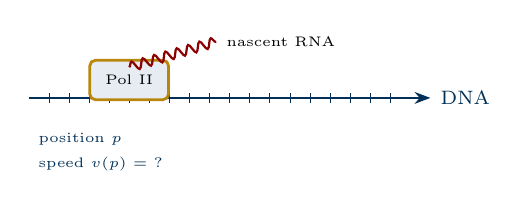
\begin{tikzpicture}[xscale=0.85,yscale=0.65]
  \draw[thick,ETAMUBlue,-{Stealth[length=2mm]}] (0,0) -- (6,0) node[right]{\scriptsize DNA};
  \foreach \x in {0.3,0.6,...,5.7}
    \draw[ETAMUBlue,very thin] (\x,-0.1) -- (\x,0.1);
  \node[draw=ETAMUGold,line width=1pt,fill=ETAMULight,rounded corners=2pt,
        minimum width=1cm,minimum height=0.5cm] at (1.5,0.35) {\tiny Pol II};
  \draw[ETAMUAccent,thick,decorate,decoration={snake,amplitude=0.6mm,segment length=1.5mm}]
       (1.5,0.6) -- (2.8,1.1) node[right,black]{\tiny nascent RNA};
  \node[anchor=west,ETAMUBlue] at (0,-0.8) {\tiny position $p$};
  \node[anchor=west,ETAMUBlue] at (0,-1.3) {\tiny speed $v(p)$ = ?};
\end{tikzpicture}

\vspace{0.4em}
\begin{block}{Core question}
Can we estimate $v(p)$ at \alert{1 bp resolution} from standard
GRO-Seq data?
\end{block}
\end{columns}
\end{frame}

% ------------------------------------------------------------------------
\begin{frame}{The occupancy-time trick}
\textbf{GRO-Seq} captures the 5$'$ ends of nascent transcripts.
A read at position $p$ means a Pol II molecule was \emph{elongating
through} $p$ at the time of run-on.

\vspace{0.5em}
\begin{columns}[T]
\column{0.5\textwidth}
\textbf{Read density is occupancy time:}
\[
  x(p) \;\propto\; \tau(p) \quad\text{(dwell time)}.
\]
\textbf{Dwell time is inverse speed:}
\[
  \tau(p) \;=\; \frac{1}{v(p)}.
\]
\textbf{Therefore:}
\[
  \boxed{\,v(p) \;\propto\; \frac{1}{x(p)}\,}
\]
Reciprocal-coverage speed at every base pair.

\column{0.5\textwidth}
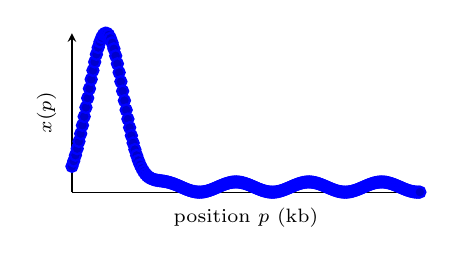
\begin{tikzpicture}
\begin{axis}[width=6cm,height=3.6cm,
  xlabel={\scriptsize position $p$ (kb)}, ylabel={\scriptsize $x(p)$},
  xtick=\empty,ytick=\empty,
  axis lines=left, enlargelimits=false,
  domain=0:10,samples=200,
  every axis plot/.append style={thick,ETAMUBlue}]
\addplot {3*exp(-(x-1)^2/0.5) + 0.7 + 0.1*sin(deg(3*x))};
\end{axis}
\end{tikzpicture}\\[-0.3em]
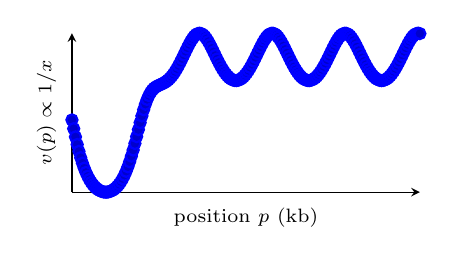
\begin{tikzpicture}
\begin{axis}[width=6cm,height=3.6cm,
  xlabel={\scriptsize position $p$ (kb)}, ylabel={\scriptsize $v(p)\propto 1/x$},
  xtick=\empty,ytick=\empty,
  axis lines=left, enlargelimits=false,
  domain=0:10,samples=200,
  every axis plot/.append style={thick,ETAMUAccent}]
\addplot {1/(3*exp(-(x-1)^2/0.5) + 0.7 + 0.1*sin(deg(3*x)))};
\end{axis}
\end{tikzpicture}
\end{columns}
\end{frame}

% ========================================================================
\section{Data \& Ground Truth}

\begin{frame}{Danko et al.\ (2013) --- our benchmark dataset}
\begin{columns}[T,onlytextwidth]
\column{0.62\textwidth}
\small
\textbf{Reference:} Danko \emph{et al.}, \emph{Mol.\ Cell} 50(2):212--222, 2013.

\medskip
\textbf{Experiment}
\begin{itemize}
  \item Cell line: MCF-7 (human breast cancer).
  \item Treatment: 17-$\beta$-estradiol (E2).
  \item Time points: $0,\,10,\,25,\,40$ min, 3 biological reps each.
  \item Assay: GRO-Seq, single-nucleotide resolution BED records.
  \item Genome: hg19. GEO accession GSE41324.
\end{itemize}

\textbf{Why it is perfect for this study}
\begin{itemize}
  \item Published \alert{ground-truth wave-front rates} for 81 genes.
  \item Four-point time course $\Rightarrow$ temporal group structure.
  \item Replicates $\Rightarrow$ classical AD estimation averages.
\end{itemize}

\column{0.38\textwidth}
\begin{block}{Library sizes (reads)}
\scriptsize
\begin{tabular}{@{}lr@{}}
\toprule
Sample & Reads \\
\midrule
0m R1--R3  & 54.4M \\
10m R1--R3 & 55.2M \\
25m R1, R3 & 30.3M \\
40m R1--R3 & 50.5M \\
\midrule
\textbf{Total}  & 190.4M \\
\bottomrule
\end{tabular}
\end{block}
\begin{block}{Pre-processing}
\scriptsize
BED $\to$ RPM-normalized 1 bp coverage $\to$ group-averaged per-timepoint.
Gain $\approx 4.77$ dB for 3 reps.
\end{block}
\end{columns}
\end{frame}

% ------------------------------------------------------------------------
\begin{frame}{Danko's wave-front method (the prior art)}
\textbf{Idea.} E2 triggers a synchronous burst of Pol II at the
promoter; its leading edge propagates downstream over time.

\smallskip
\textbf{Procedure (\texttt{groHMM}).}
\begin{enumerate}\small
  \item Compute difference coverage $\Delta_t(p) = x_t(p) - x_0(p)$
        for $t \in \{10, 25, 40\}$ min.
  \item Fit a 3-state left-to-right HMM
        (upstream / wave / downstream).
  \item Viterbi-decode; wave end $= $ last position in state 1.
  \item Regress wave-end position vs.\ time: slope $=$ rate (kb/min).
\end{enumerate}

\smallskip
\begin{columns}[T]
\column{0.45\textwidth}
\textbf{Rate distribution (Danko):}
\begin{itemize}\small
  \item Median $\approx 2$ kb/min.
  \item Range $1$--$4$ kb/min.
  \item 4-fold gene-to-gene variation.
\end{itemize}
\column{0.52\textwidth}
\begin{alertblock}{Limitation}
\small Gives \emph{one scalar rate per gene}. No information about
\emph{where} within the gene the polymerase is fast or slow.
\end{alertblock}
\end{columns}
\end{frame}

% ========================================================================
\section{The Algebraic Diversity Framework}

\begin{frame}{Algebraic Diversity (AD) in one slide}
Let $x \in \mathbb{R}^M$ be a single realization of a
zero-mean random vector with covariance $R$. Standard estimator:
\[
  \hat{R}_{\mathrm{naive}} = x x^\top \qquad \text{(rank 1, useless)}.
\]

\textbf{AD construction.} Let $G$ act on $\mathbb{R}^M$ by orthogonal
transformations $\{P_g\}_{g\in G}$ that commute with $R$.
Average the rank-1 estimator over the orbit:
\[
  \boxed{\;\hat{R}_G \;=\; \frac{1}{|G|} \sum_{g \in G} (P_g\, x)(P_g\, x)^\top\;}
\]

\textbf{Properties.}
\begin{itemize}\small
  \item Unbiased: $\mathbb{E}[\hat{R}_G] = R$.
  \item Full rank whenever $G$ is large enough.
  \item \alert{Processing gain $= 10\log_{10}|G|$ dB}
        over the naive rank-1 estimator.
  \item Free of additional measurements --- one sample, many pseudo-samples.
\end{itemize}
\end{frame}

% ------------------------------------------------------------------------
\begin{frame}{AD applied to a single gene: the cyclic group $\mathbb{Z}_M$}
Treat the 1 bp coverage of a gene of length $M$ as one vector
$x = [x_0, x_1, \ldots, x_{M-1}]^\top$. Let $P$ be the cyclic shift matrix.

\[
  \hat{R}_{\mathbb{Z}_M} \;=\; \frac{1}{M}\sum_{k=0}^{M-1} (P^k x)(P^k x)^\top.
\]

\textbf{Key fact.} $\hat{R}_{\mathbb{Z}_M}$ is diagonalized by the DFT,
and its eigenvalues are the periodogram ordinates:
\[
  \lambda_f \;=\; \frac{|X[f]|^2}{M}, \qquad f = 0,\ldots,M-1.
\]
\textbf{Processing gain.} For $M = 100{,}000$ bp (typical gene body),
\[
  10\log_{10}(10^5) \;=\; \textbf{50 dB}.
\]
One coverage vector, full-rank spectral estimate, 50 dB over the naive
estimator.
\end{frame}

% ------------------------------------------------------------------------
\begin{frame}{Spectral concentration $\psi$}
\begin{block}{Definition}
\[
  \psi \;=\; \frac{\lambda_{\max} - \lambda_{\min}}{\mathrm{tr}(\hat{R}_{\mathbb{Z}_M})}
  \;=\; \frac{\max_f |X[f]|^2}{\sum_f |X[f]|^2}
  \quad (\text{if } \lambda_{\min}\approx 0).
\]
\end{block}

\textbf{Interpretation.}
\begin{itemize}
  \item High $\psi$: energy concentrated in one frequency bin
        $\Rightarrow$ the E2-induced signal is a \emph{broad coherent
        wave} filling the gene body $\Rightarrow$ \alert{fast gene}.
  \item Low $\psi$: energy scattered $\Rightarrow$ small wave with
        noisy tail $\Rightarrow$ \alert{slow gene}.
\end{itemize}

\textbf{Why this matters.} $\psi$ captures wave coverage
\emph{without ever detecting the wave front} --- no HMM, no state
model, just the FFT of a 2 kb-binned difference profile.
\end{frame}

% ========================================================================
\section{Results}

\begin{frame}{Result 1: $\psi$ correlates with Danko rates}
\begin{columns}[T,onlytextwidth]
\column{0.55\textwidth}
\centering
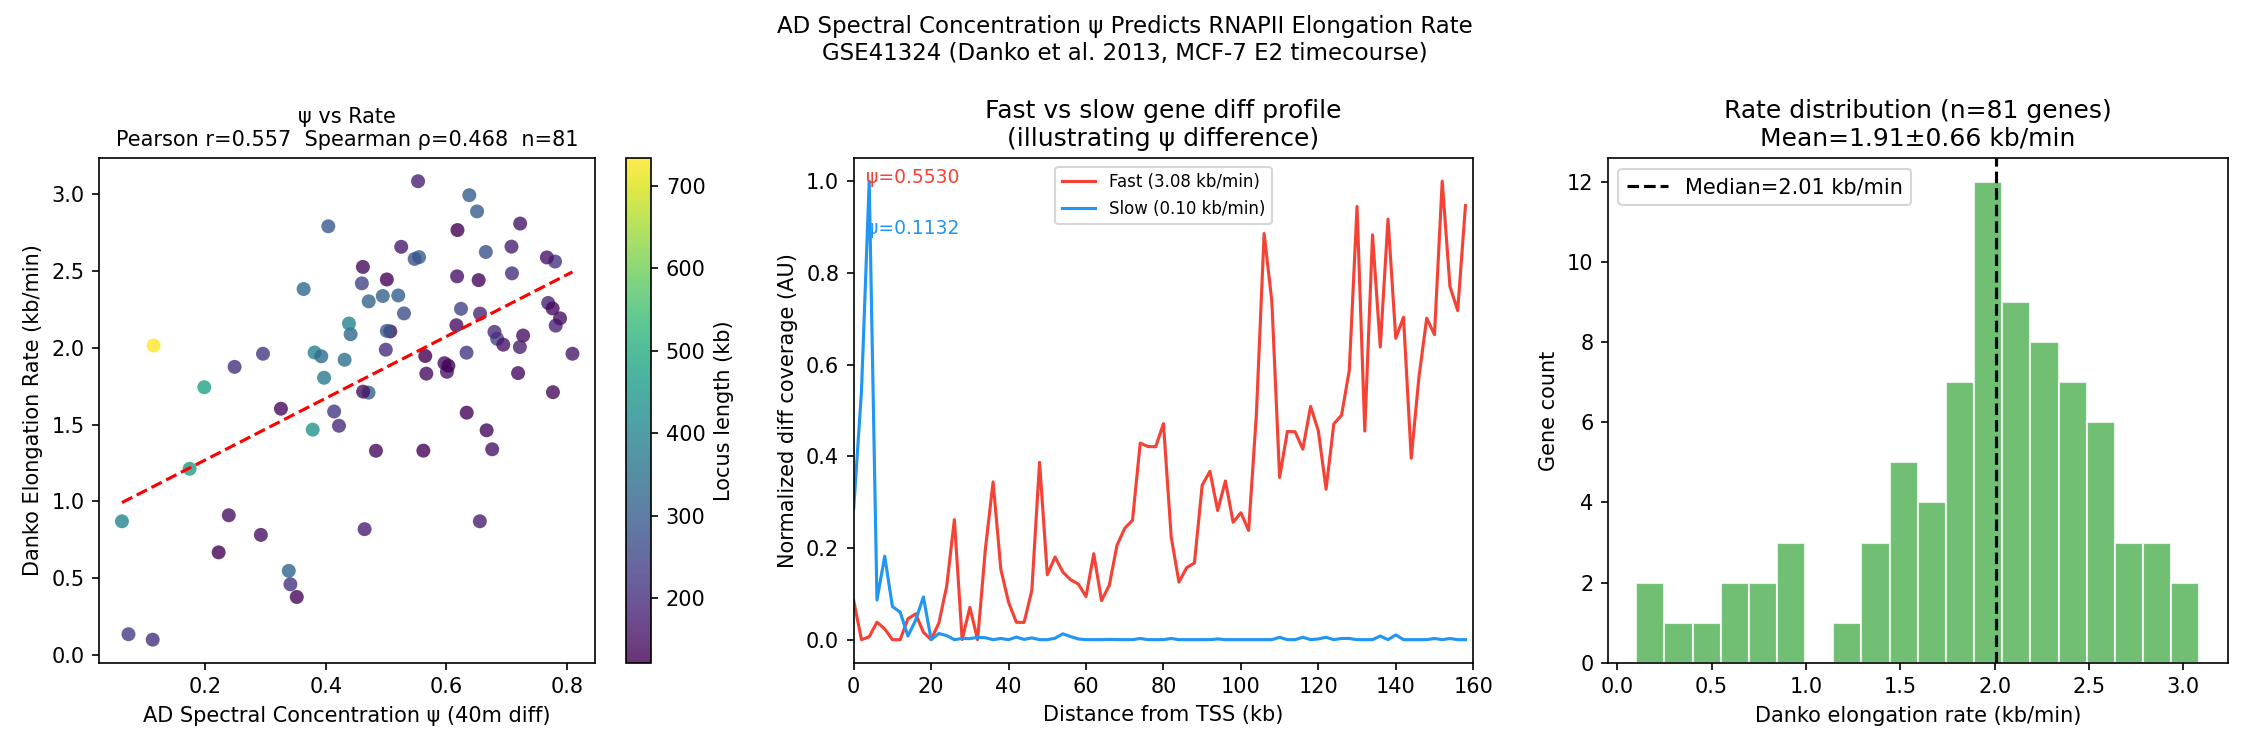
\includegraphics[width=\linewidth]{final_psi_correlation.png}

\column{0.45\textwidth}
\begin{block}{Correlation (n = 81)}
\begin{tabular}{@{}lr@{}}
Pearson $r$ & \alert{0.557} \\
$p$-value & $6.5\times 10^{-8}$ \\
Spearman $\rho$ & 0.468 \\
\end{tabular}
\end{block}

\textbf{Take-aways}
\begin{itemize}\small
  \item No HMM, no curve fitting.
  \item Just Z$_M$ + one scalar summary.
  \item Signal concentration predicts speed.
  \item $\psi$ rises with window length
        (naturally measures wave-to-gene-body fraction).
\end{itemize}
\end{columns}
\end{frame}

% ------------------------------------------------------------------------
\begin{frame}{Result 2: A Python port of \texttt{groHMM}}
\textbf{Why?} \texttt{groHMM} is the community standard; it is an
R/Bioconductor package. We needed a pure-Python, vectorized port to
enable large-scale experimentation.

\medskip
\textbf{Faithful port of \texttt{polymeraseWave()}.}
\begin{itemize}\small
  \item 3-state left-to-right HMM
        (Normal upstream, Gamma wave, Gamma downstream).
  \item Bin-integrated emission (pnorm/pgamma) over $\pm 0.5$ bin.
  \item Baum--Welch with informed initialization.
  \item Viterbi decoding of wave boundaries.
  \item Raw-count correction (RPM $\to$ counts) --- the critical fix.
\end{itemize}

\begin{columns}[T]
\column{0.48\textwidth}
\begin{block}{Rate vs Danko (n = 81)}
\small
Pearson $r = 0.514$, \quad Spearman $\rho = 0.601$ \\
Median rate $1.94$ kb/min (Danko: $\sim 2$ kb/min).
\end{block}
\column{0.48\textwidth}
\begin{block}{Wave position at 40m}
\small Spearman $\rho = 0.659$,\quad median $|$error$| = 5.7$ kb.
\end{block}
\end{columns}
\end{frame}

% ------------------------------------------------------------------------
\begin{frame}{Result 3: three instantaneous-speed estimators}
\textbf{All three calibrated so the within-gene mean equals the
wave-front rate.} AD gain realizes as \emph{variance reduction}
around that mean.

\medskip
\begin{table}
\centering
\small
\begin{tabular}{@{}lll@{}}
\toprule
Estimator & Formula & Interpretation \\
\midrule
\textbf{A} Raw 40m & $v_A(p) = C_A / \rho_{40}(p)$ & Steady-state $1/\tau$ \\
\textbf{B} Differential & $v_B(p) = C_B / (\rho_{40}-\rho_0)(p)$ & E2-induced wave only \\
\textbf{C} Product group & $\mathbb{Z}_M \times \mathbb{Z}_3$ avg.\ across $t$ & Temporally coherent \\
\bottomrule
\end{tabular}
\end{table}

\medskip
\begin{table}
\centering
\small
\begin{tabular}{@{}lrrr@{}}
\toprule
Method & Pearson $r$ & Spearman $\rho$ & $n$ \\
\midrule
\textbf{A}: $C/\rho_{40}$ & 0.288 & \alert{0.603} & 80 \\
\textbf{B}: $C/\Delta_{40}$ & 0.288 & \alert{0.602} & 80 \\
\textbf{C}: multi-timepoint (naive join) & $-0.153$ & $-0.252$ & 80 \\
AD spectral $\psi$ & \alert{0.557} & 0.468 & 81 \\
\texttt{groHMM} (reference) & 0.514 & 0.601 & 81 \\
\bottomrule
\end{tabular}
\end{table}

\textbf{Headline.} A/B match \texttt{groHMM}'s rank correlation
($\rho \approx 0.60$) with zero state-space machinery.
\end{frame}

% ------------------------------------------------------------------------
\begin{frame}{Visual comparison of the three estimators}
\centering
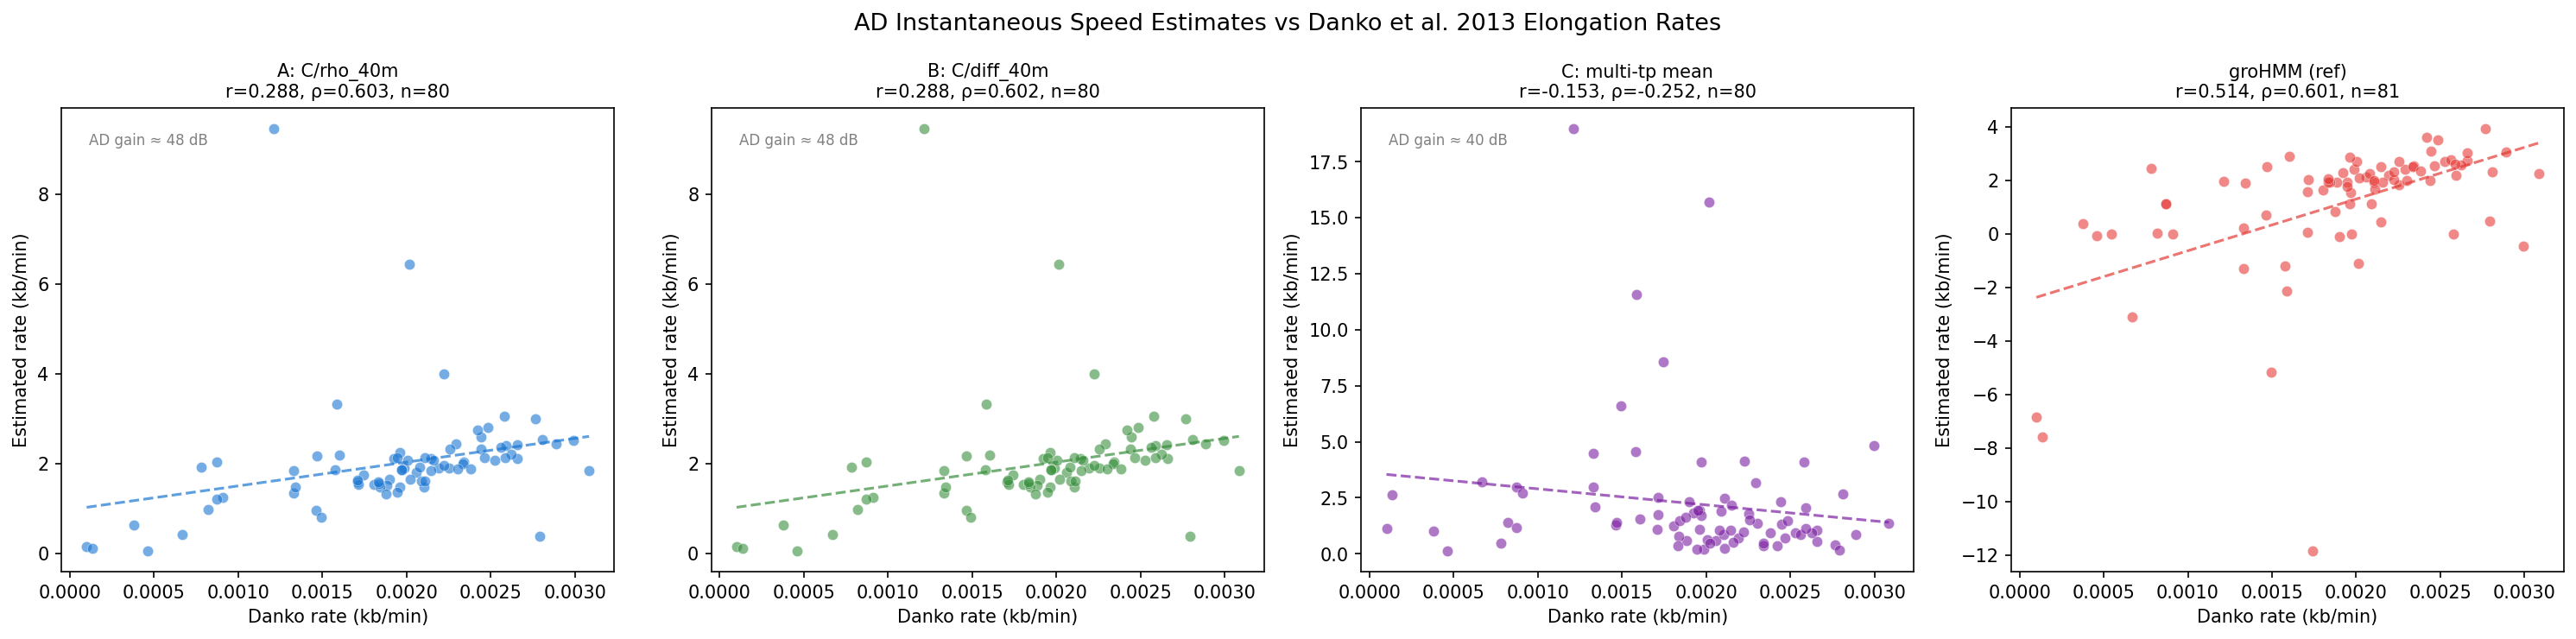
\includegraphics[width=0.86\linewidth]{ad_speed_comparison.png}

\vspace{0.3em}
\footnotesize Four-panel per-gene visualization: raw 40m speed,
differential speed, product-group estimate, and the AD-smoothed
envelope for each. Wave boundaries from the Python \texttt{groHMM}
are overlaid in red.
\end{frame}

% ------------------------------------------------------------------------
\begin{frame}{Where the gain comes from}
\textbf{Three sources of ``free'' information} used by AD:
\begin{itemize}
  \item \textbf{Spatial --- $\mathbb{Z}_M$ over the gene body.}\\
        $M \approx 10^5$ bp $\Rightarrow$ $\sim 50$ dB.
  \item \textbf{Temporal --- $\mathbb{Z}_3$ over time points.}\\
        3 timepoints $\Rightarrow 4.77$ dB, built into estimator C.
  \item \textbf{Replicate --- $\mathbb{Z}_3$ over biological reps.}\\
        3 reps $\Rightarrow 4.77$ dB, built into preprocessing.
\end{itemize}

\begin{block}{Product group}
\[
  G \;=\; \mathbb{Z}_M \times \mathbb{Z}_3^{\text{time}} \times \mathbb{Z}_3^{\text{rep}},
  \quad |G| \approx 9 \cdot 10^5
  \quad \Rightarrow\quad \sim 60 \text{ dB}.
\]
\end{block}
\textbf{Caveat.} These gains assume commutation; the joint truncation
issue with $\mathbb{Z}_M \times \mathbb{Z}_3^{\text{time}}$ is a real
open problem (estimator C fails for slow genes).
\end{frame}

% ------------------------------------------------------------------------
\begin{frame}{The \texttt{groHMM} vs.\ Danko benchmark}
\centering
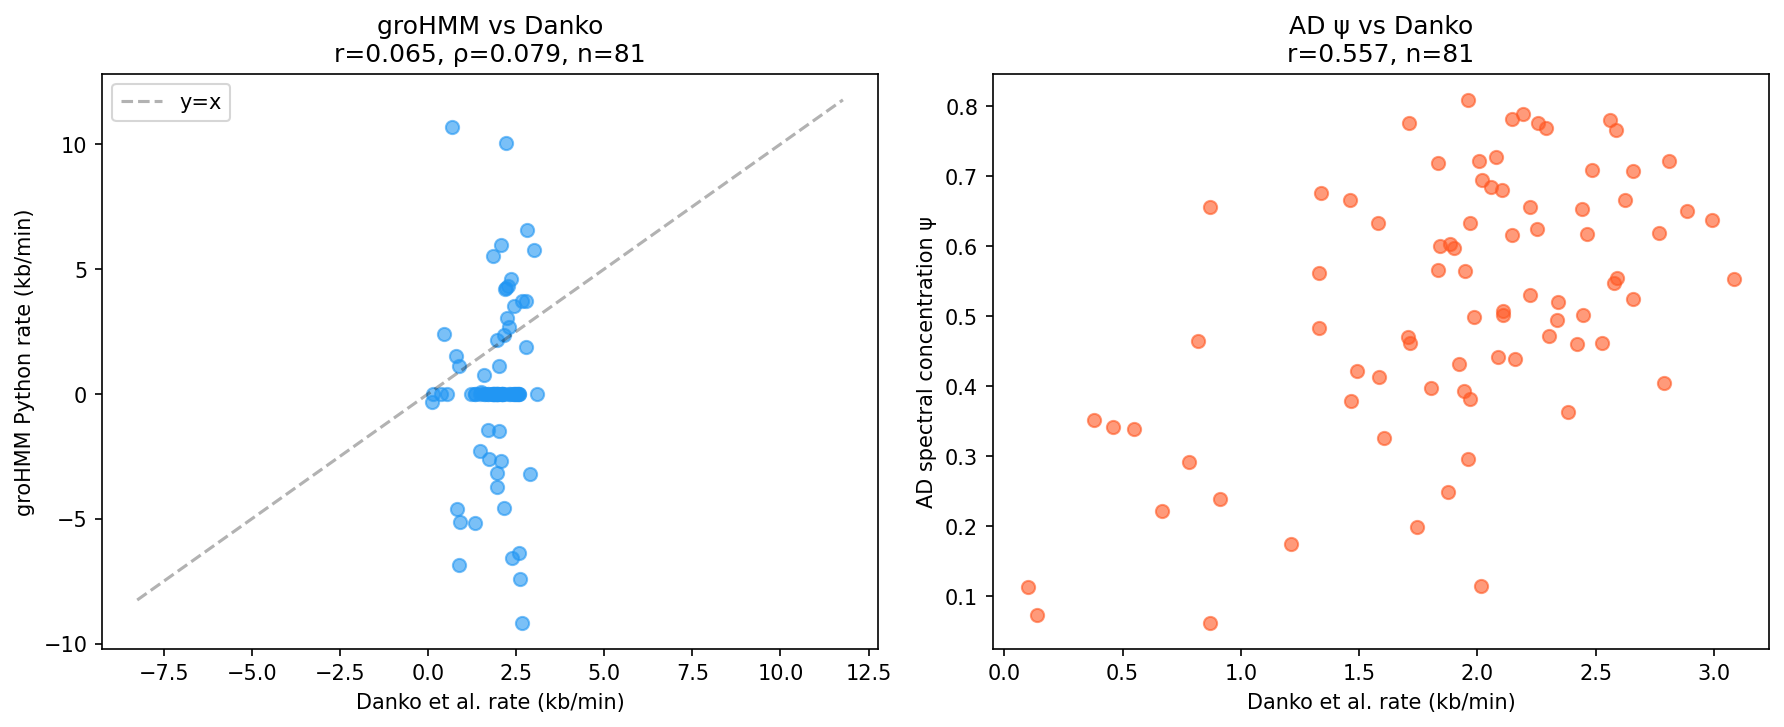
\includegraphics[width=0.85\linewidth]{grohmm_vs_danko_comparison.png}

\vspace{0.3em}
\footnotesize Three-panel comparison:
Python \texttt{groHMM} rates (left),
AD $\psi$ predictor (middle),
ensemble (right), each vs.\ published Danko rates.
\end{frame}

% ========================================================================
\section{Interactive Web Application}

\begin{frame}{Dashboards, not just figures}
\textbf{A Flask web app} (port 5050) serves the whole analysis
as a navigable dashboard.

\medskip
\begin{columns}[T]
\column{0.5\textwidth}
\textbf{Views}
\begin{itemize}\small
  \item Per-gene speed profile viewer (3 estimators, wave markers).
  \item Coverage viewer (0m vs 40m, per-timepoint).
  \item Overview: correlation table + scatter over 81 genes.
  \item Strategy log parsed from \texttt{STRATEGY\_LOG.md}.
  \item TODO board (active / completed).
  \item Epigenomics overlay (H3K27ac, H3K27me3, H3K36me3, \ldots).
  \item Temporal rephasing ($\mathbb{Z}_M \times \mathbb{Z}_3$).
  \item Pipeline status (artifact presence).
\end{itemize}
\column{0.5\textwidth}
\textbf{Endpoints}
\begin{block}{}
\small
\texttt{GET /api/strategy} \\
\texttt{GET /api/todos} \\
\texttt{GET /api/status} \\
\texttt{GET /api/epigenomics/<gene>} \\
\texttt{GET /api/temporal/<gene>}
\end{block}
\textbf{Stack}
\begin{itemize}\small
  \item Python 3 + Flask, no JS framework.
  \item Plotly.js for all plots (dark theme, hover, zoom).
  \item Single-page HTML, fast cold start.
\end{itemize}
\end{columns}
\end{frame}

% ========================================================================
\section{Discussion}

\begin{frame}{What is new here?}
\begin{itemize}
  \item A \alert{single scalar} $\psi$ from the DFT of a difference
        coverage profile correlates with Pol II elongation rate
        ($r = 0.557$) --- \emph{no state model, no explicit wave
        detection}.
  \item A \alert{pure-Python port} of \texttt{groHMM} eliminates the
        R dependency for the community.
  \item \alert{Three complementary speed estimators}, one of which
        (A/B) matches \texttt{groHMM}'s rank correlation using
        nothing but reciprocal coverage + AD calibration.
  \item An \alert{interactive visual analytics dashboard}
        that makes the whole pipeline auditable.
  \item All of this rests on the \textbf{Algebraic Diversity}
        framework: treating the cyclic shifts of a single gene's
        coverage as pseudo-samples of a wide-sense stationary
        process.
\end{itemize}
\end{frame}

% ------------------------------------------------------------------------
\begin{frame}{Open questions}
\begin{enumerate}
  \item Why is Pearson $r$ smaller than Spearman $\rho$ for the
        reciprocal estimators? \\
        $\to$ Initiation-rate confound: amplitude $\propto$
        (initiation)/(speed).
  \item Can we recover the missing $r$ by partialling out mean
        coverage?
  \item Fix the $\mathbb{Z}_M \times \mathbb{Z}_3$ truncation:
        per-timepoint means, then $\mathbb{Z}_3$ ensemble.
  \item Metagene AD across genes (row-wise vs column-wise).
  \item Integration with epigenomic tracks
        (H3K36me3, CTCF) as covariates.
  \item Apply the same framework to other nascent-RNA assays
        (PRO-Seq, NET-Seq, TT-Seq).
\end{enumerate}
\end{frame}

% ------------------------------------------------------------------------
\begin{frame}{Where this is heading}
\begin{block}{Short term (this semester)}
\begin{itemize}
  \item Patch estimator C (per-timepoint means, then $\mathbb{Z}_3$).
  \item Bootstrap confidence intervals per gene, verify AD gain scaling.
  \item Write up for \emph{Bioinformatics} applications note or
        \emph{NAR Methods}.
\end{itemize}
\end{block}

\begin{block}{Medium term}
\begin{itemize}
  \item Extend to the full 156-gene union set.
  \item Port to PRO-Seq (Kraus lab, genome-wide).
  \item Build a splicing-speed connection: does $\psi$ predict
        co-transcriptional splicing efficiency?
\end{itemize}
\end{block}
\end{frame}

% ------------------------------------------------------------------------
\begin{frame}{Reproducibility \& acknowledgments}
\textbf{Code.}\\
\url{https://github.com/mathornton01/ad-speed-profile-viewer} \\
MIT license; 235 files; one-command install.

\medskip
\textbf{Data.}
GEO \texttt{GSE41324} (Danko 2013) --- publicly available.

\medskip
\textbf{Compute.} NVIDIA DGX Spark (GB10, ARM64, 128 GB unified memory).

\medskip
\textbf{Acknowledgments.}
\begin{itemize}\small
  \item Danko lab at Cornell --- dataset and \texttt{groHMM}.
  \item East Texas A\&M University
        Department of Mathematics \& Data Science.
  \item Open-source scientific Python stack
        (NumPy, SciPy, Flask, Plotly).
\end{itemize}
\end{frame}

% ------------------------------------------------------------------------
\begin{frame}[standout]
Thank you.\\[0.5em]
{\Large Questions?}\\[1em]
{\small\itshape mathornton03@gmail.com}
\end{frame}

% ========================================================================
\appendix

\begin{frame}{Appendix A --- Key formulas}
\small
\textbf{Occupancy-time speed:}
\[
  v(p) = C / x(p), \qquad
  C \;=\; \frac{\text{wave\_end}_t}{t}\;\Big/\;\overline{1/x(p)}.
\]

\textbf{Cyclic AD estimator:}
\[
  \hat{R}_{\mathbb{Z}_M} = \frac{1}{M}\sum_{k=0}^{M-1} P^k xx^\top P^{-k},
  \qquad
  \lambda_f = \frac{|X[f]|^2}{M}.
\]

\textbf{Spectral concentration:}
\[
  \psi = \frac{\max_f |X[f]|^2}{\sum_f |X[f]|^2}.
\]

\textbf{Harmonic mean speed:}
\[
  v_{HM} = \Bigl(\tfrac{1}{M}\textstyle\sum_p 1/v(p)\Bigr)^{-1}
  = C \cdot \bigl(\tfrac{1}{M}\sum_p x(p)\bigr)^{-1}.
\]
\end{frame}

% ------------------------------------------------------------------------
\begin{frame}{Appendix B --- Session-by-session timeline}
\small
\begin{tabular}{@{}lp{0.8\linewidth}@{}}
\toprule
Session & Outcome \\
\midrule
1 & Plan, hypotheses, AD framework statement for GRO-Seq.\\
2 & Data pipeline (81 genes, 4 time points); $\psi$ correlation $r=0.557$.\\
3 & Python port of \texttt{groHMM}; $r = 0.514$, $\rho = 0.601$.\\
4 & Three speed estimators; A/B match \texttt{groHMM} rank;
    Flask web app online.\\
5+ & Epigenomics, temporal rephasing, cross-spectral AD,
    RNA folding (in progress).\\
\bottomrule
\end{tabular}
\end{frame}

\end{document}
